\newcommand{\triangOK}{\textcolor[rgb]{00,0.45,0.10}{$\blacktriangle$}}
\newcommand{\triangBAD}{\textcolor[rgb]{0.7,00,00}{$\blacktriangledown$}}
\newcommand{\ball}{\textcolor[rgb]{0.7,0.70,0.0}{$\bullet$}}
 	
%\begin{table}
%\centering
%\caption{}
%\label{tab::}
%\begin{footnotesize}
%\toprule
%Tabela
%\midrule
%\bottomrule
%\end{footnotesize}
%\end{table}

\chapter{Experimentos}
\label{cap::experimentos}


Nesse capítulo relataremos os diversos experimentos efetuados e seus resultados.
Decidimos por realizar a seguinte divisão: 
na Seção~\ref{sec::preliminares} abordamos os pontos em comum de todos os experimentos e mostramos as bases de dados usadas,
%já na Seção~\ref{sec::fitness} avaliamos três possibilidades para a função de \textit{fitness} do Programa Genético,
enquanto, nas Seções~\ref{sec::documentos}, \ref{sec::categorias} e \ref{sec::bioinfo} abordamos a classificação de atributos textuais, categóricos e numéricos, respectivamente.

\section{Preliminares}
\label{sec::preliminares}

TODO: falar das subsecoes.

\subsection{Bases de dados}

Nosso trabalho se divide em três conjuntos de bases de dados: as bases de documentos, as bases do UCI (citar) e uma base de bioinformática.

Iniciamos por mostrar a Figura \ref{fig::basesdoc}, contendo as distribuições dos exemplos das quatro bases de documentos que estamos usando. Todas as bases foram pré-processadas, com remoção de \textit{stop words}, assim como foi atribuída somente uma única classe para todos os documentos que originalmente poderiam pertencer a mais de uma.
A base de documentos digitais da \textsc{ACM}, chamada \textsc{ACM-DL} (\textit{Association for Computing Machinery Digital Library}), é um rico acerto de artigos acadêmicos da área da Ciência da Computação e mostrada na Figura \ref{fig::acm}. Utilizamos somente um subconjunto formado por 56.450 termos diferentes em 24.897 artigos divididos em 11 classes. (falar dos grafos).
A base \textit{Reuters} contém 8.184 documentos divididos em 8 classes, contendo 24.986 termos distintos. Eles são provenientes da agência de notícias com o mesmo nome da base. 
Por sua vez, a base \textit{Ohsumed} apresenta 18.302 documentos médicos, em 23 classes e 45.991 termos.
Finalmente, a base 20-\textit{newgroup} (\textsc{20ng}) contém 18.827 mensagens de texto com 110.502 termos único, enviadas para grupos de notícia de diversos assuntos como ciência, religião, entre outros, totalizando 20 classes.
Todos os pontos mostrados na Figura \ref{fig::basesdoc} são referentes à quantidade de exemplos de cada classe, ordenados de maneira crescente, da classe de menor popularidade para a de maior. Verificamos que a base \textit{20-newsgroup} é a que apresenta a distribuição mais equilibrada de exemplos por classe, enquanto a \textit{ohsumed} apresenta a pior, com 17 das 23 classes contendo menos que 1.000 exemplos por classe e com duas classes contendo mais de 2.500.

\begin{figure}[!h]
  \centering
  \subfloat[][ACM-DL]{\label{fig::acm}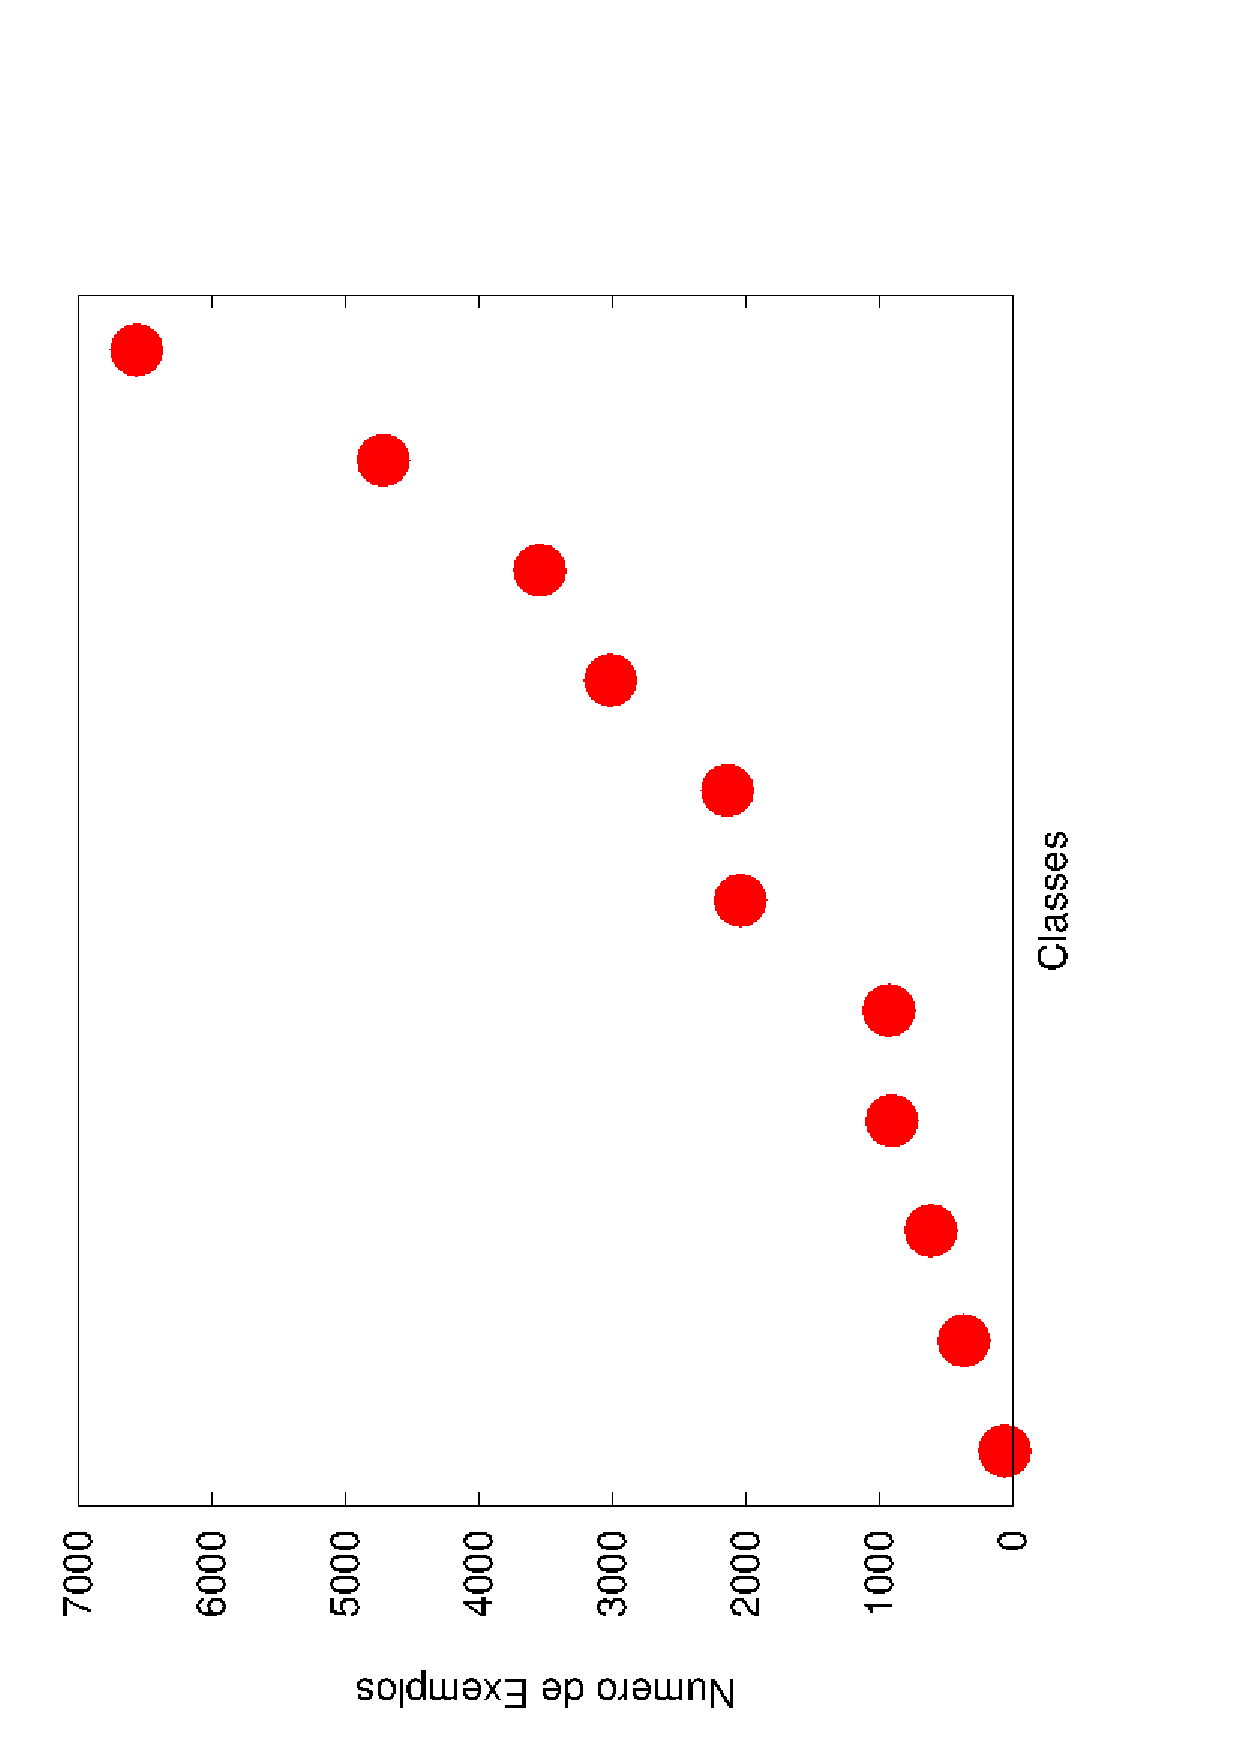
\includegraphics[angle=270, width=0.40\textwidth]{figures/perfil/acm.png}}
  \subfloat[][Reuters]{\label{fig::reuters}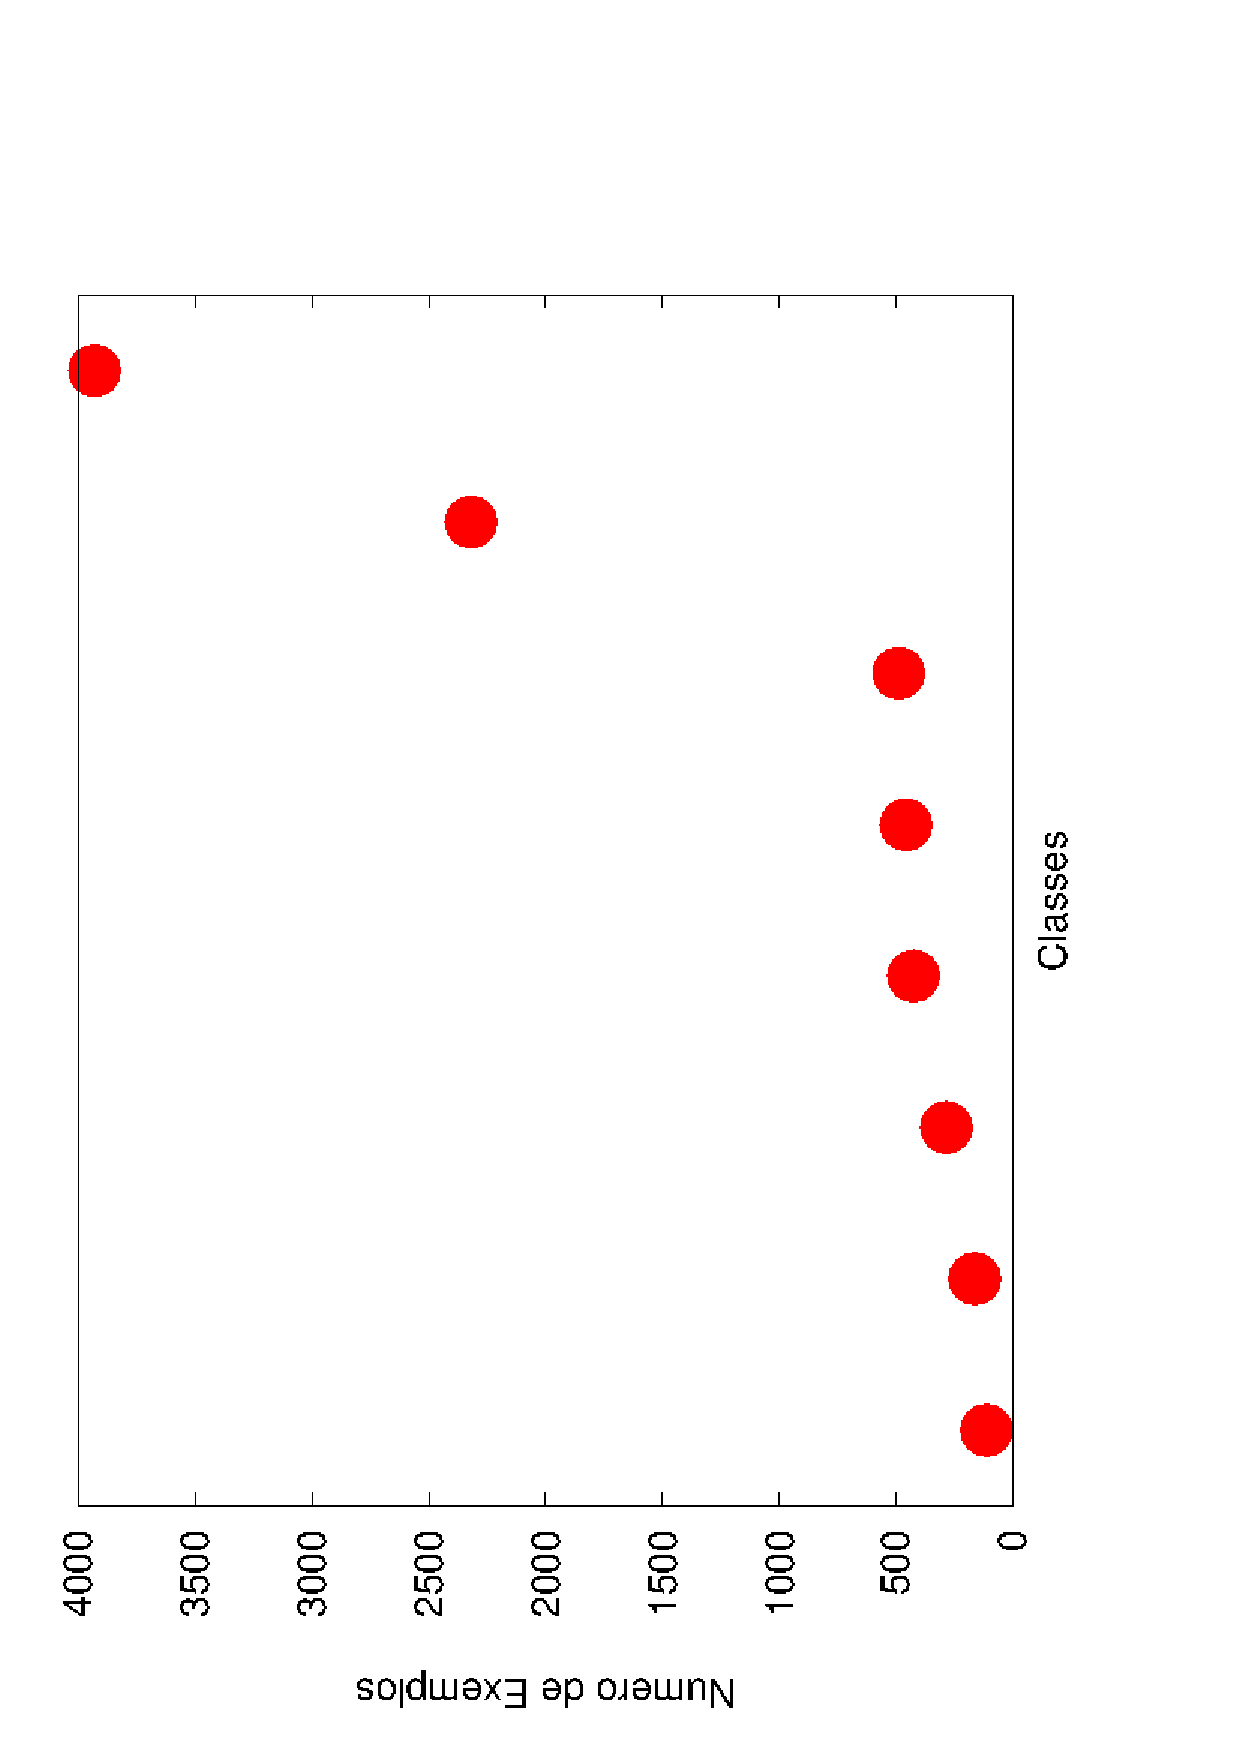
\includegraphics[angle=270, width=0.40\textwidth]{figures/perfil/reuters.png}}
    \\
  \subfloat[][Ohsumed]{\label{fig::ohsumed}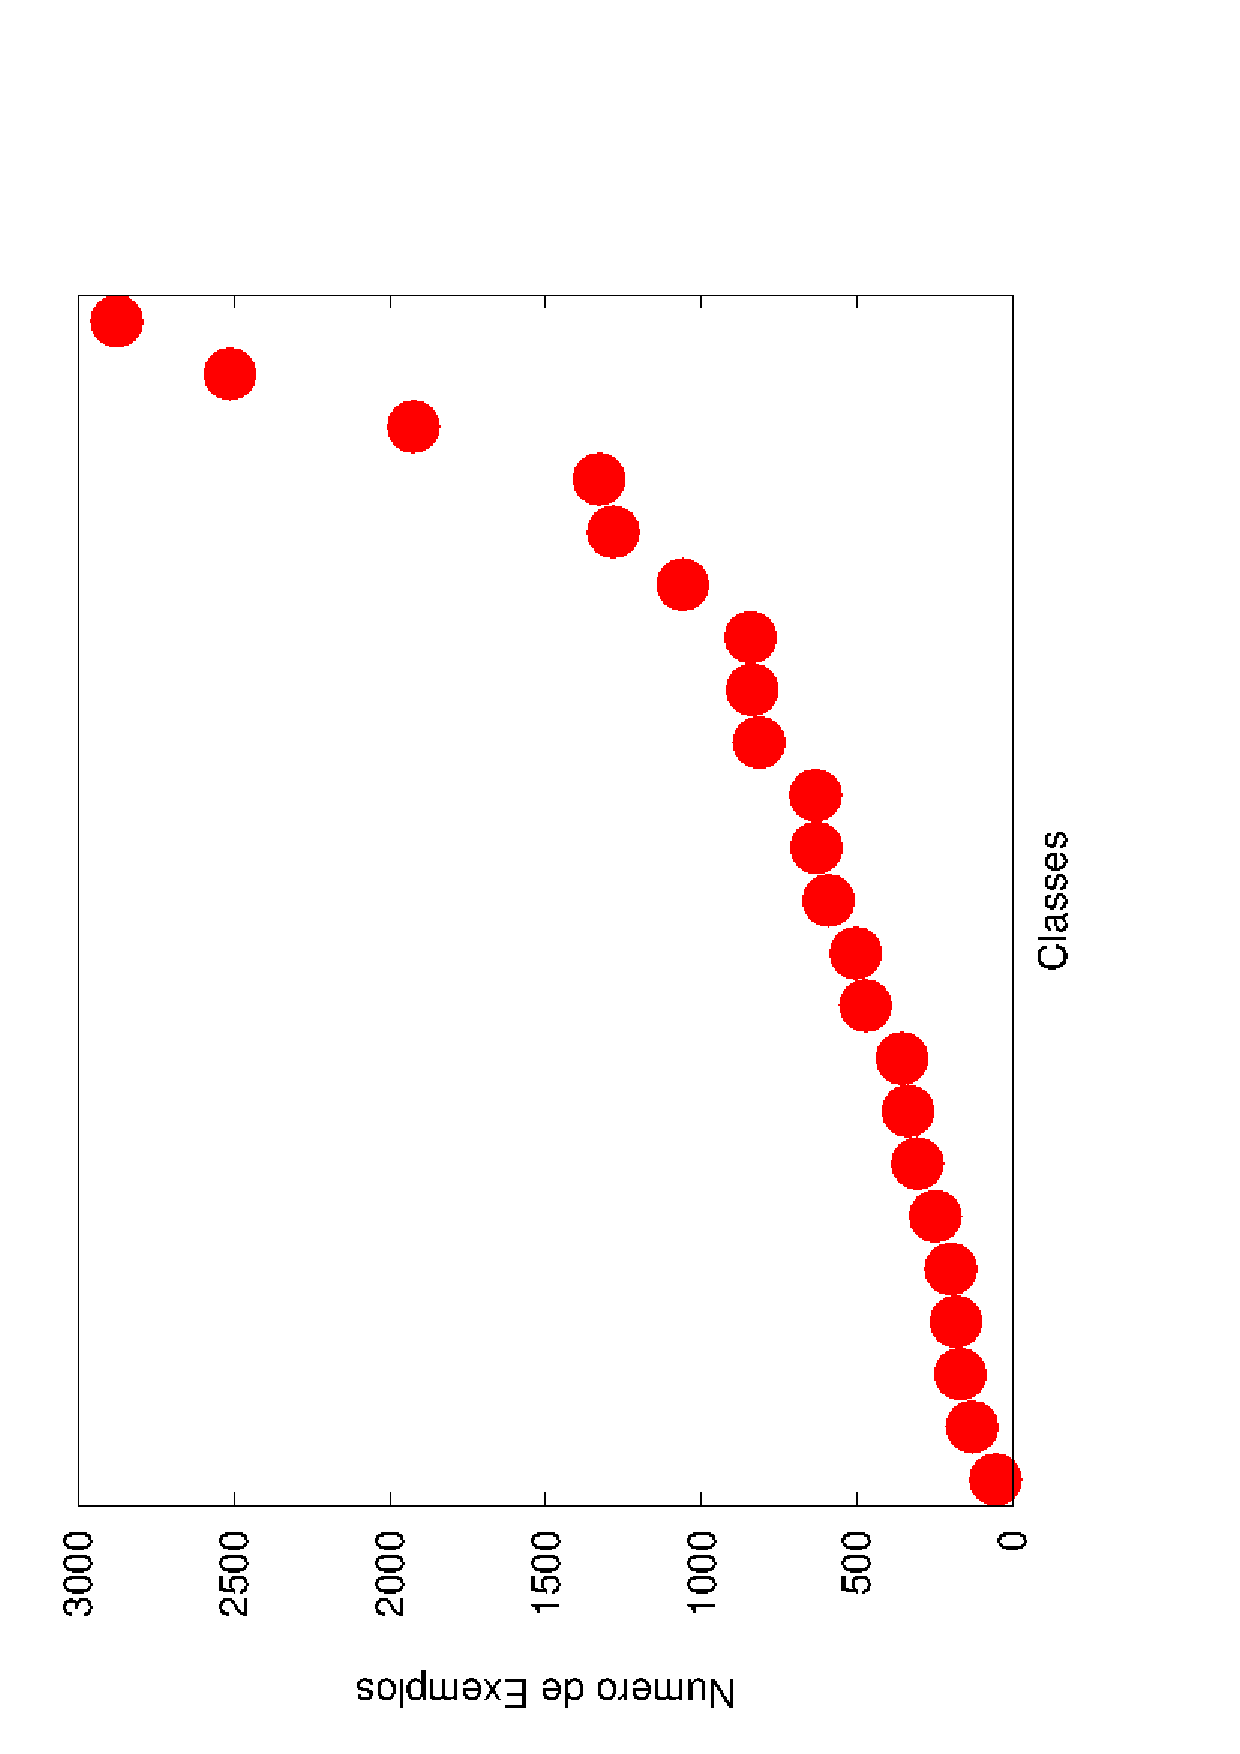
\includegraphics[angle=270, width=0.40\textwidth]{figures/perfil/ohsumed.png}}
  \subfloat[][20-NewsGroup]{\label{fig::20ng}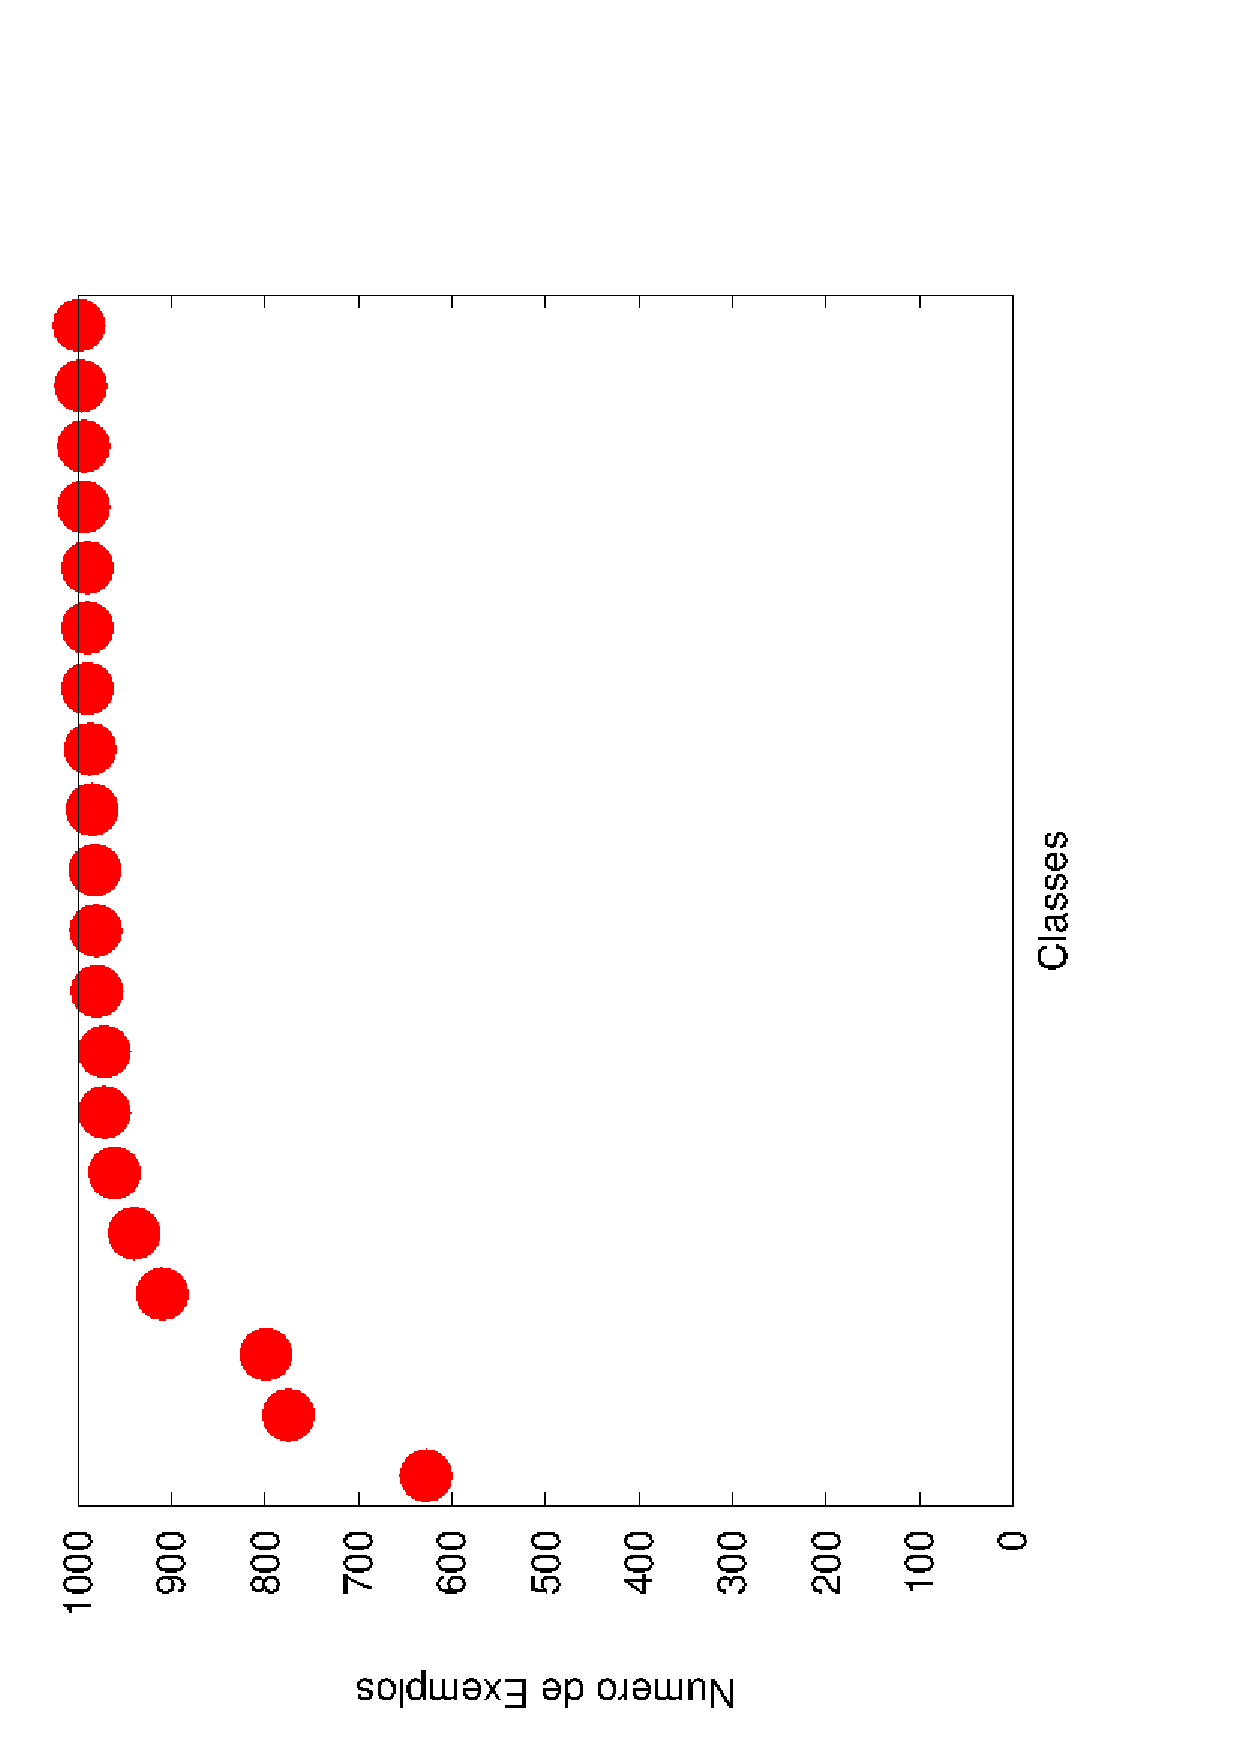
\includegraphics[angle=270, width=0.40\textwidth]{figures/perfil/20ng.png}}

\caption{Distribuição de classes nas bases de documentos.}
\label{fig::basesdoc}
\end{figure}

Na Figura \ref{fig::basesdoc}, mostramos o perfil de quatro bases do repositório de bases para aprendizagem de máquina do campos de Irvine da Univeridade da California (\textsc{UCI}) (\cite{UCI98}). Todas as bases são compostas por poucos atributos, todos categóricos, e poucas classes. A base \textit{Cars} contém 1.728 exemplos com 6 atributos cada, apresentando características importantes para decidir a condição de um carro usado entre não aceitável, aceitável, bom e muito bom. A base \textit{chess} utiliza de 36 atributos e apresenta 3.196 instâncias para decidir se a partir de alguns movimentos finais do jogo de xadrez, o jogador que joga com as peças brancas pode ganhar ou não. \textit{Nursery} é uma base formada por candidaturas para as escolas de enfermaria de Liubliana, Eslovênia. Ela é composta de 12.960 exemplos de 8 atributos que descrevem aspectos de um(a) candidato(a) para a escola de enfermaria. Cada exemplo pode ser classificado em cinco classes que vão desde não recomendado até muito recomendado, com a classe recomendado apresentando apenas dois exemplos. Por último a base \textit{tictactoe}, mostra as 958 combinações possíveis das 9 casas do jogo da velha, sendo as classes possíveis a vitória do jogador \textsc{x} ou não.

\begin{figure}[h]
  \centering
  \subfloat[][cars]{\label{fig::cars}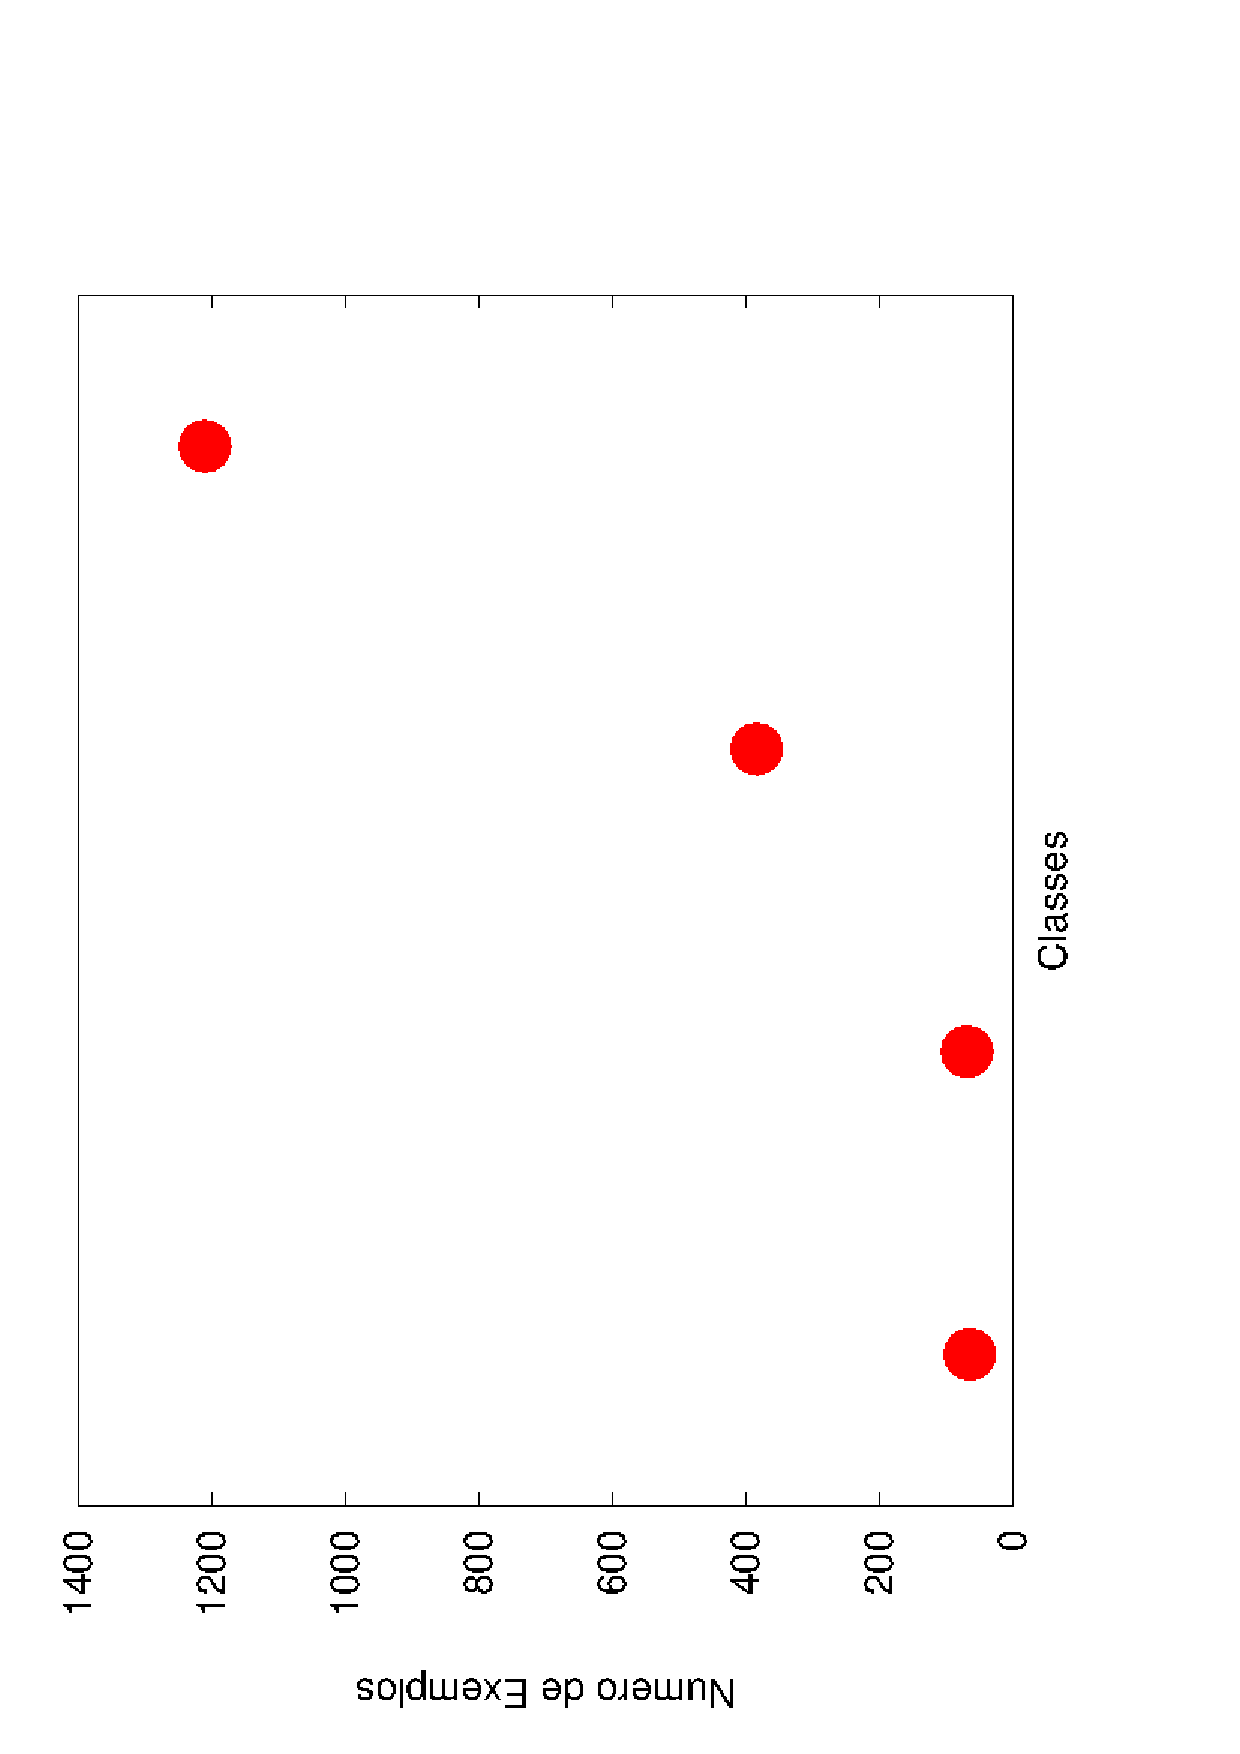
\includegraphics[angle=270, width=0.40\textwidth]{figures/perfil/cars.png}}
  \subfloat[][chess]{\label{fig::chess}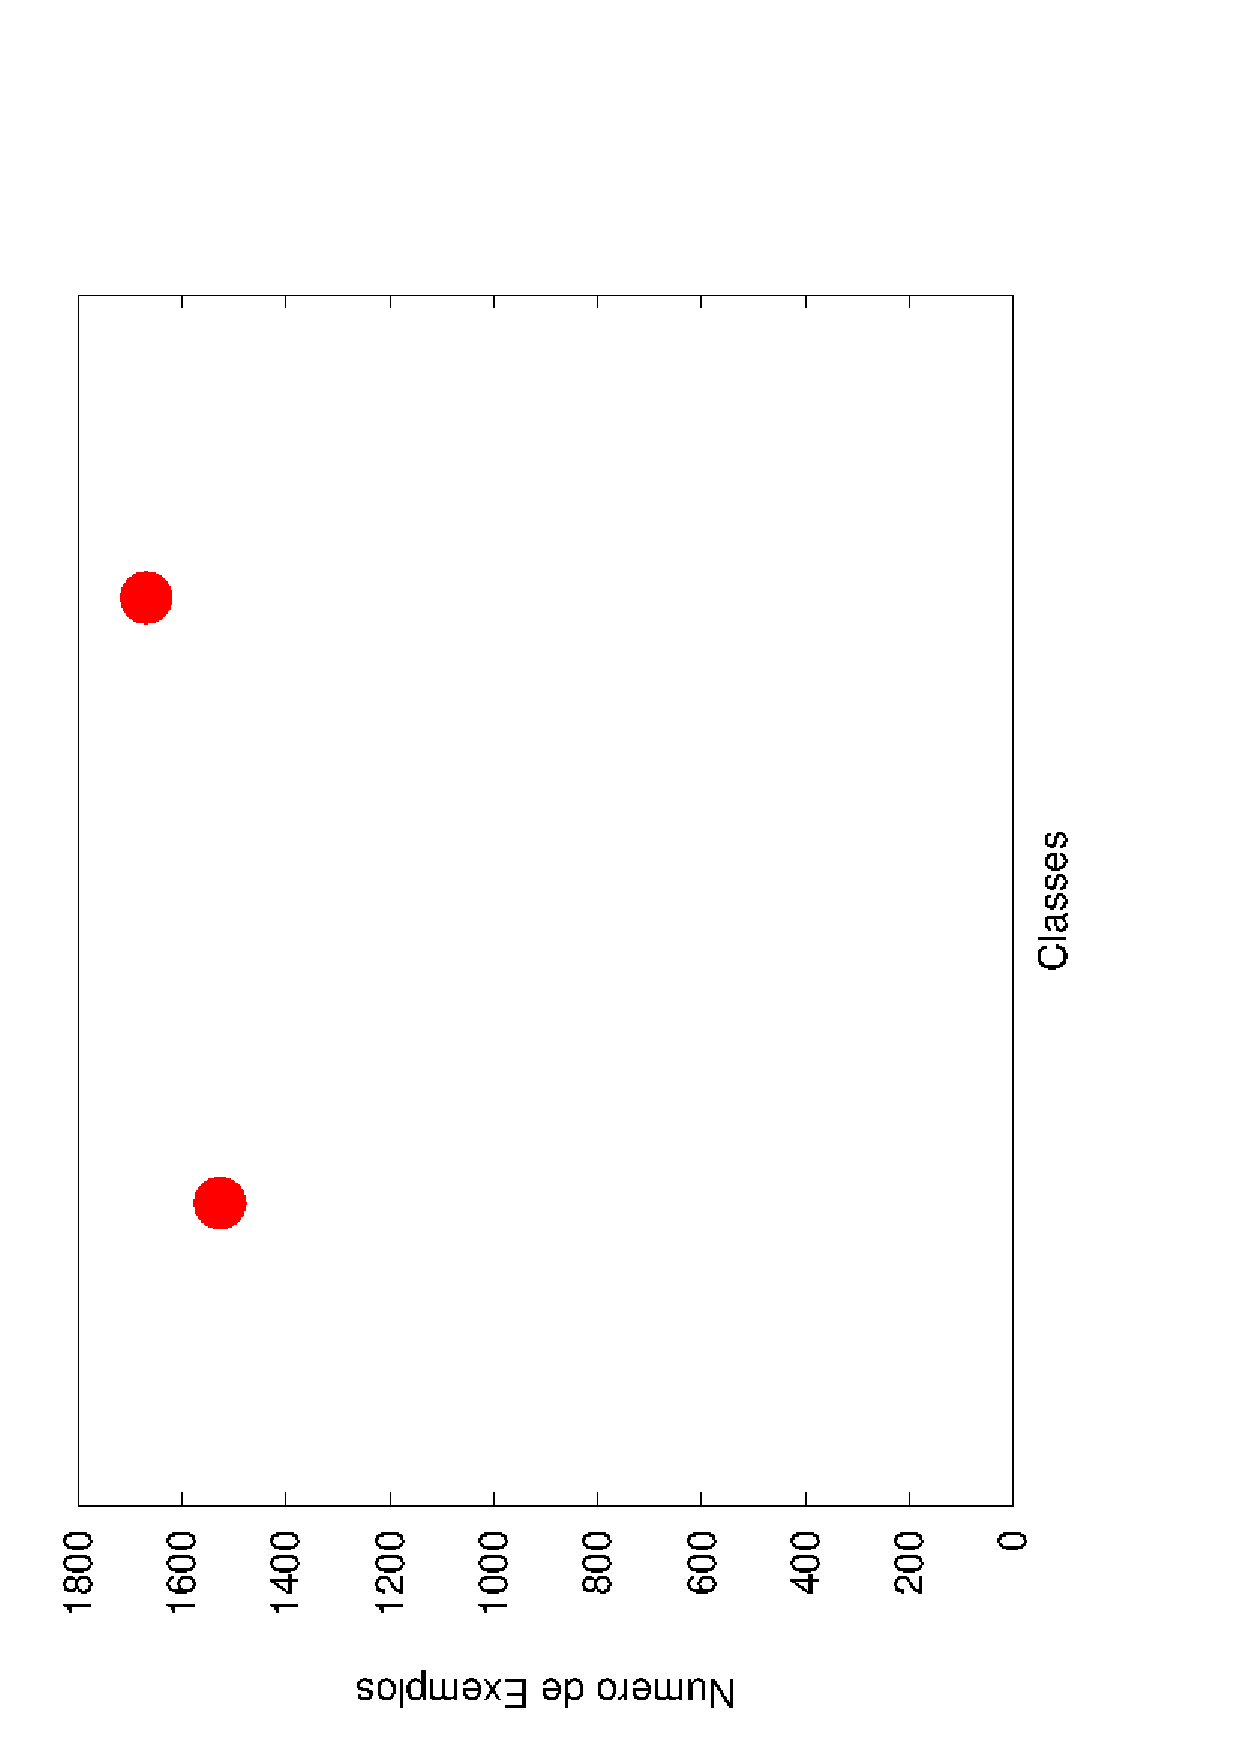
\includegraphics[angle=270, width=0.40\textwidth]{figures/perfil/chess.png}}
    \\
  \subfloat[][nursery]{\label{fig::nursery}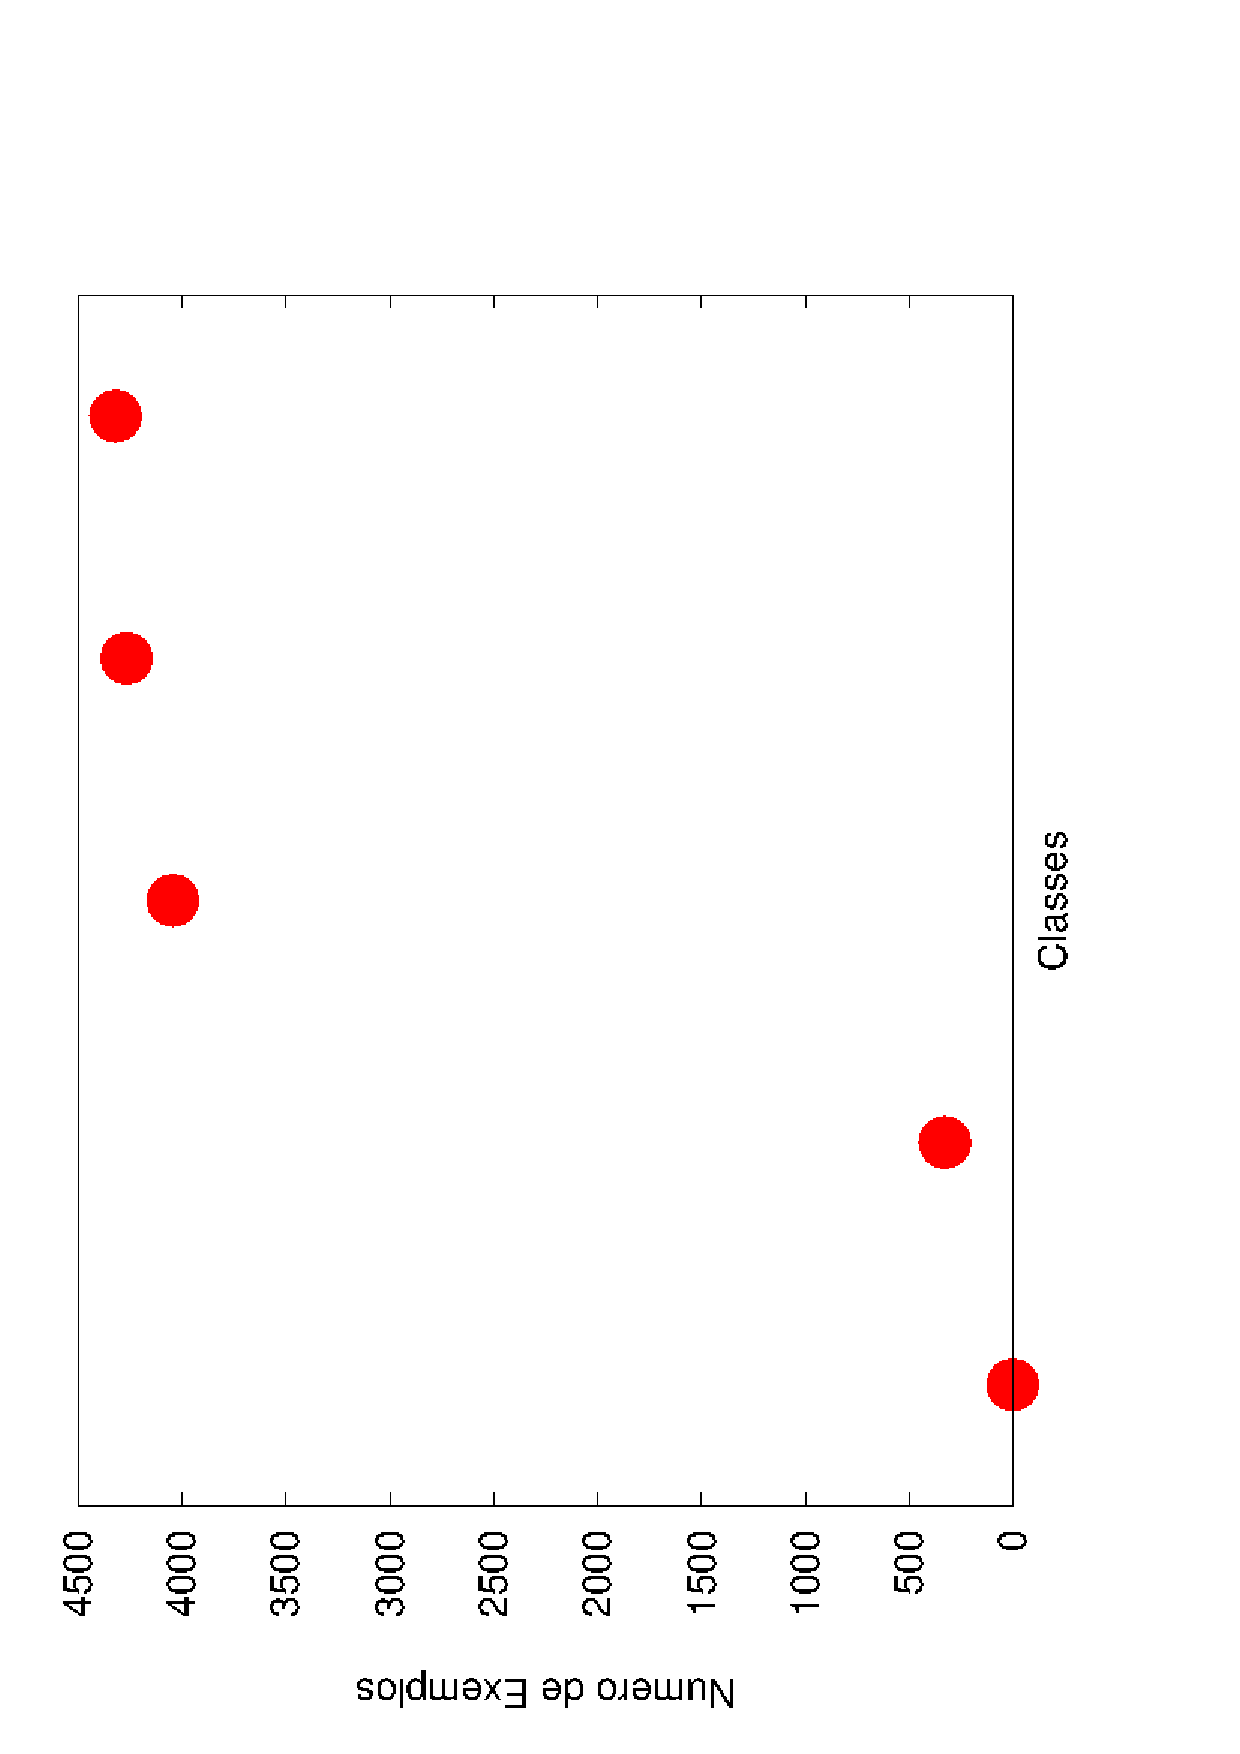
\includegraphics[angle=270, width=0.40\textwidth]{figures/perfil/nursery.png}}
  \subfloat[][tictactoe]{\label{fig::tictactoe}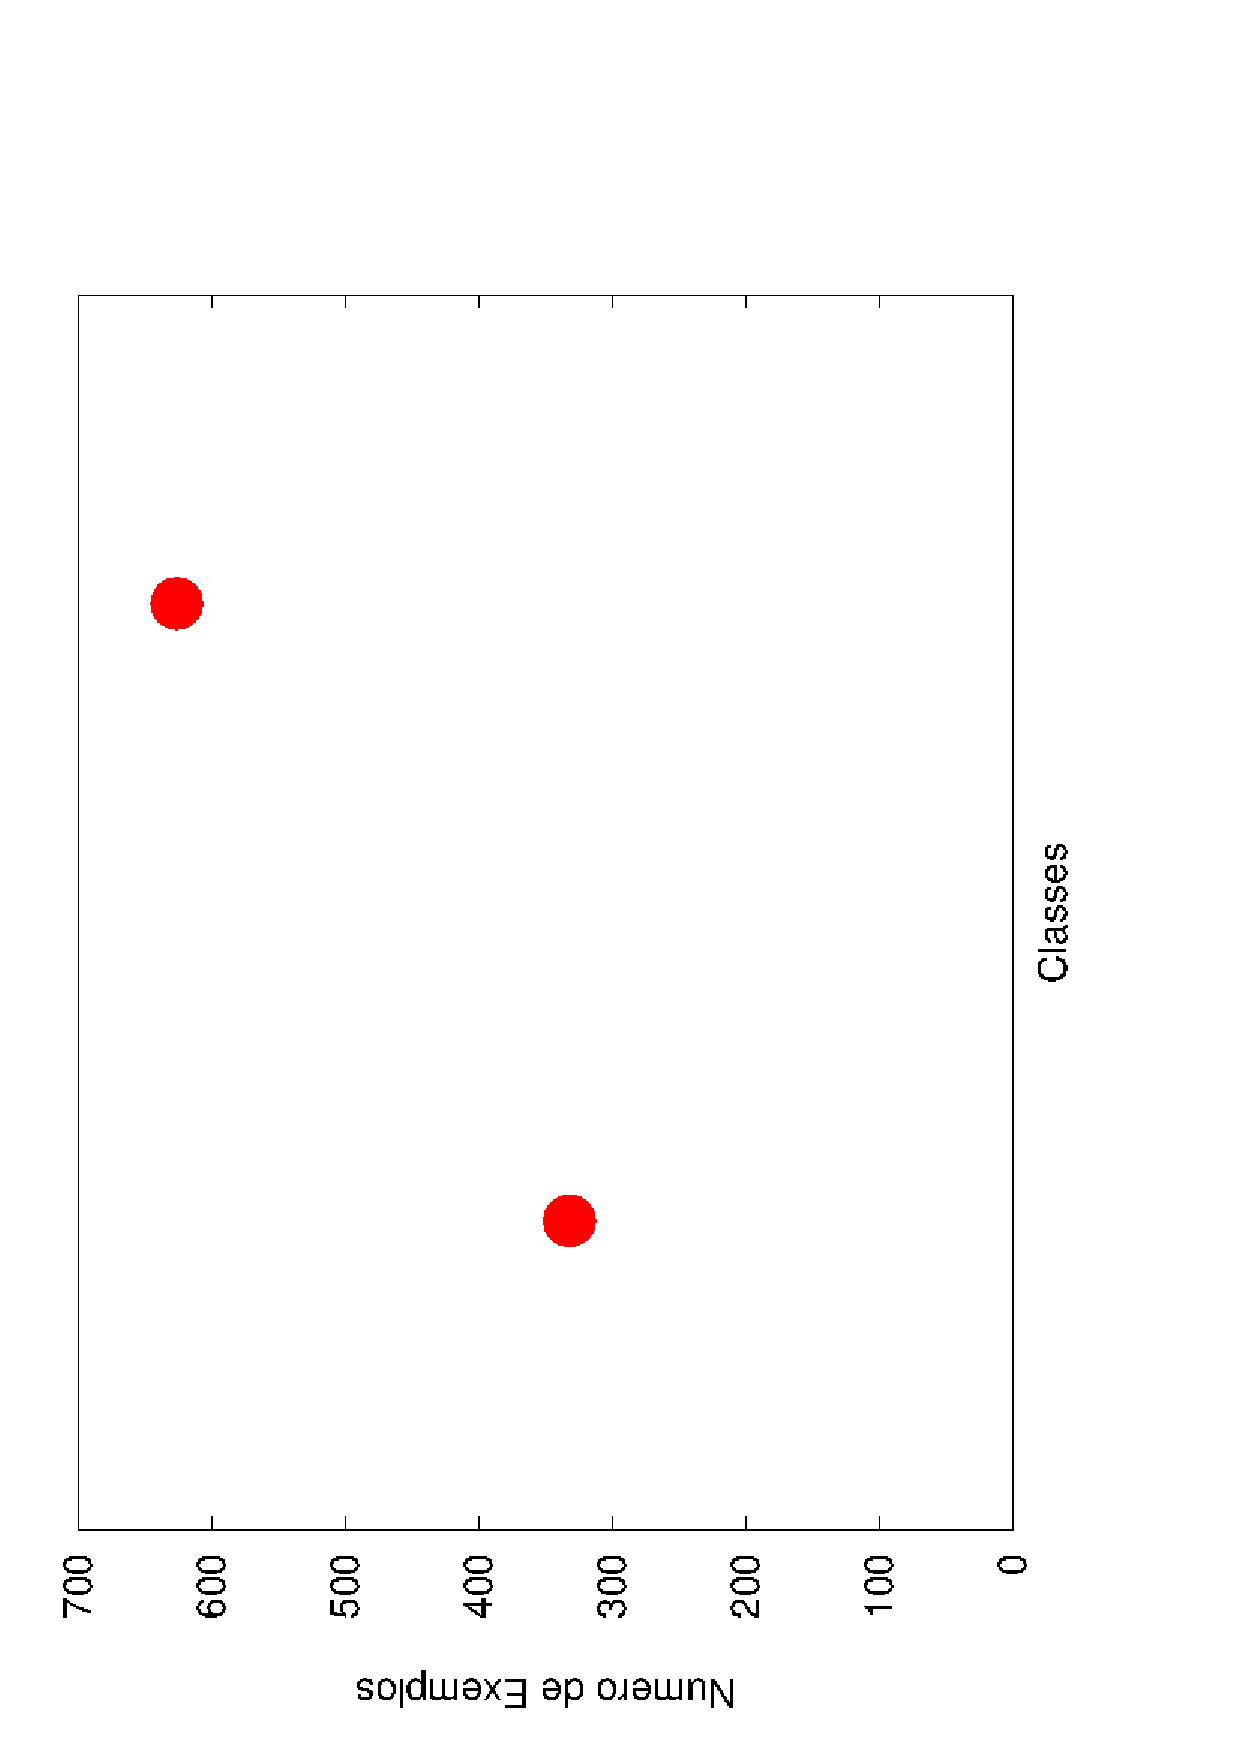
\includegraphics[angle=270, width=0.40\textwidth]{figures/perfil/tictactoe.png}}

\caption{Distribuição de classes nas bases de atributos categóricos.}
\label{fig::basescategorias}
\end{figure}

Consultar o paper do douglas para falar sobre a astral.

\begin{figure}[h]
  \centering
%  \subfloat[][Astral]{\label{fig:astral}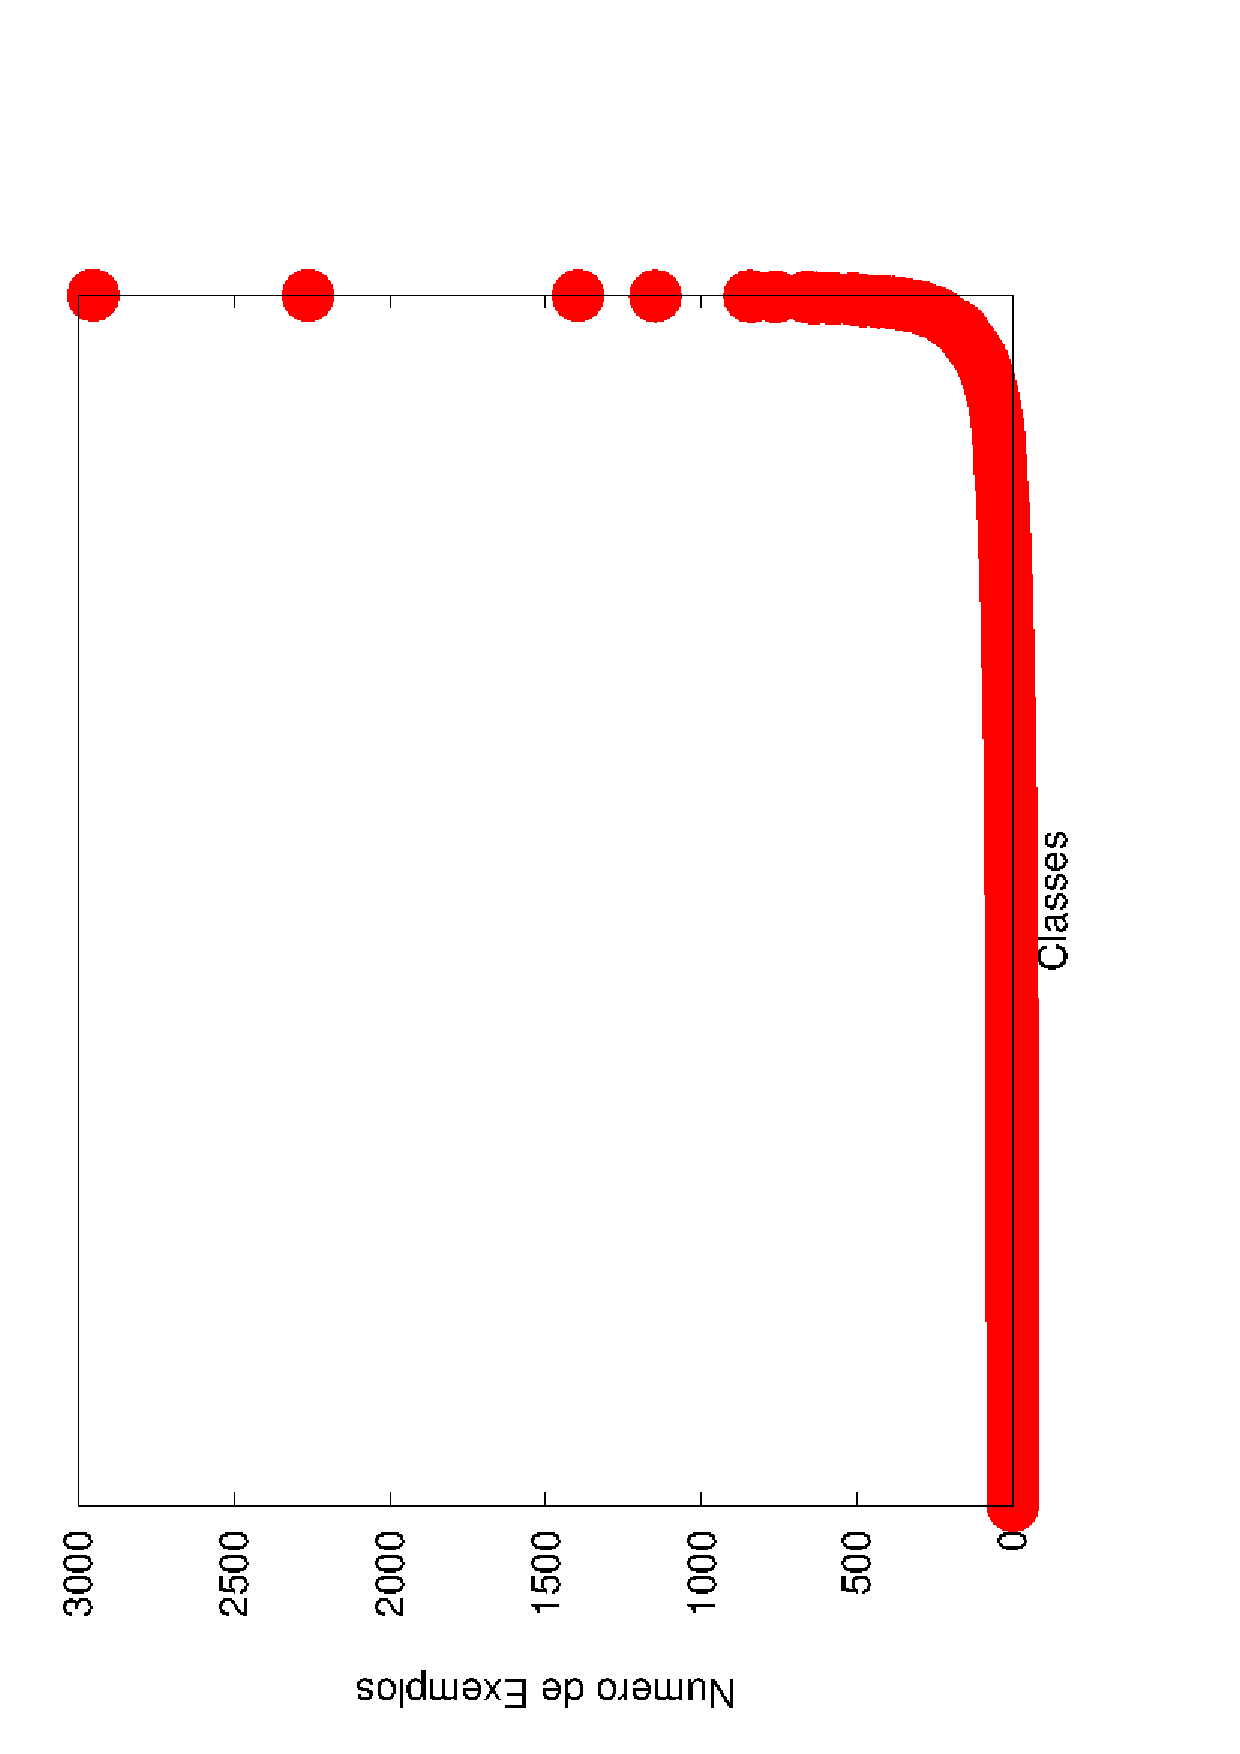
\includegraphics[angle=270, width=0.40\textwidth]{figures/perfil/astral.png}}
%  \subfloat[][Douglas]{\label{fig:douglas}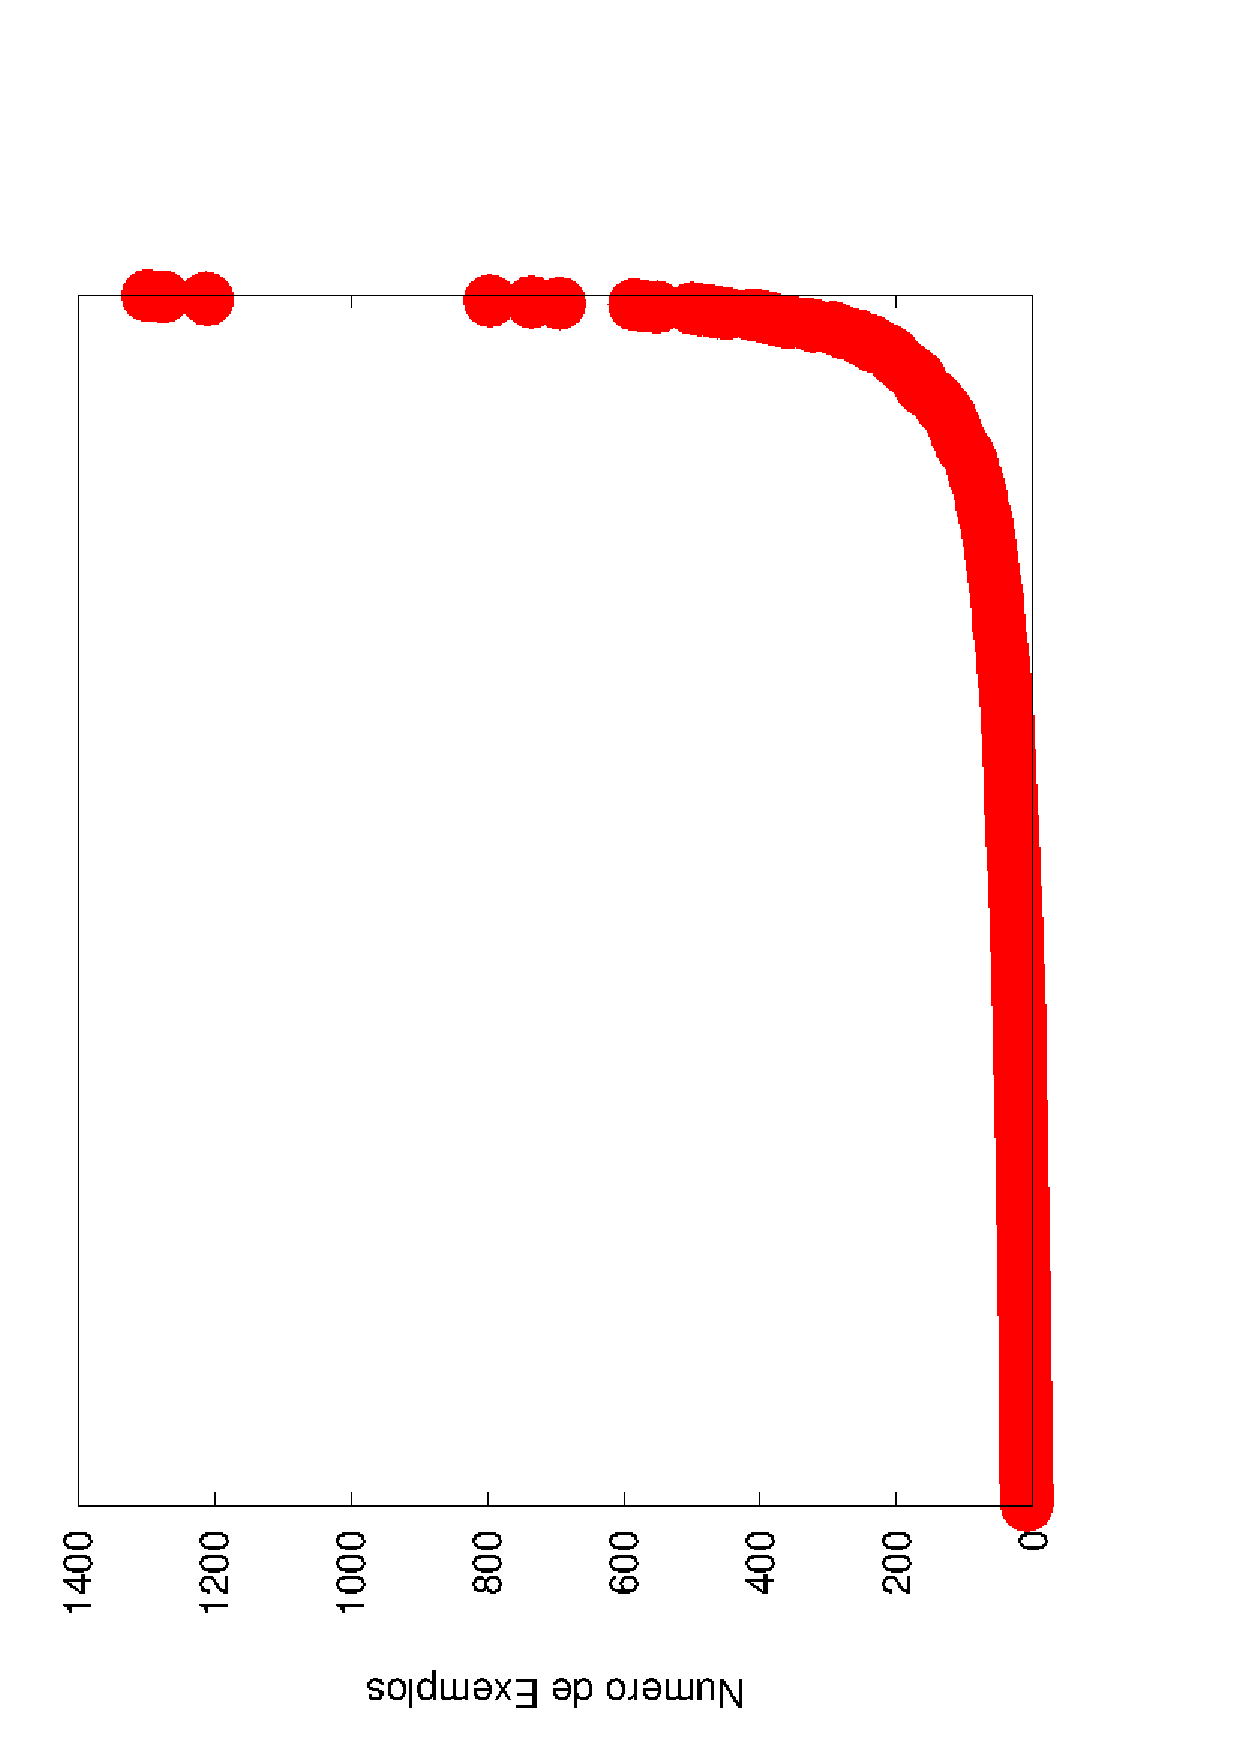
\includegraphics[angle=270, width=0.40\textwidth]{figures/perfil/douglas.png}}
  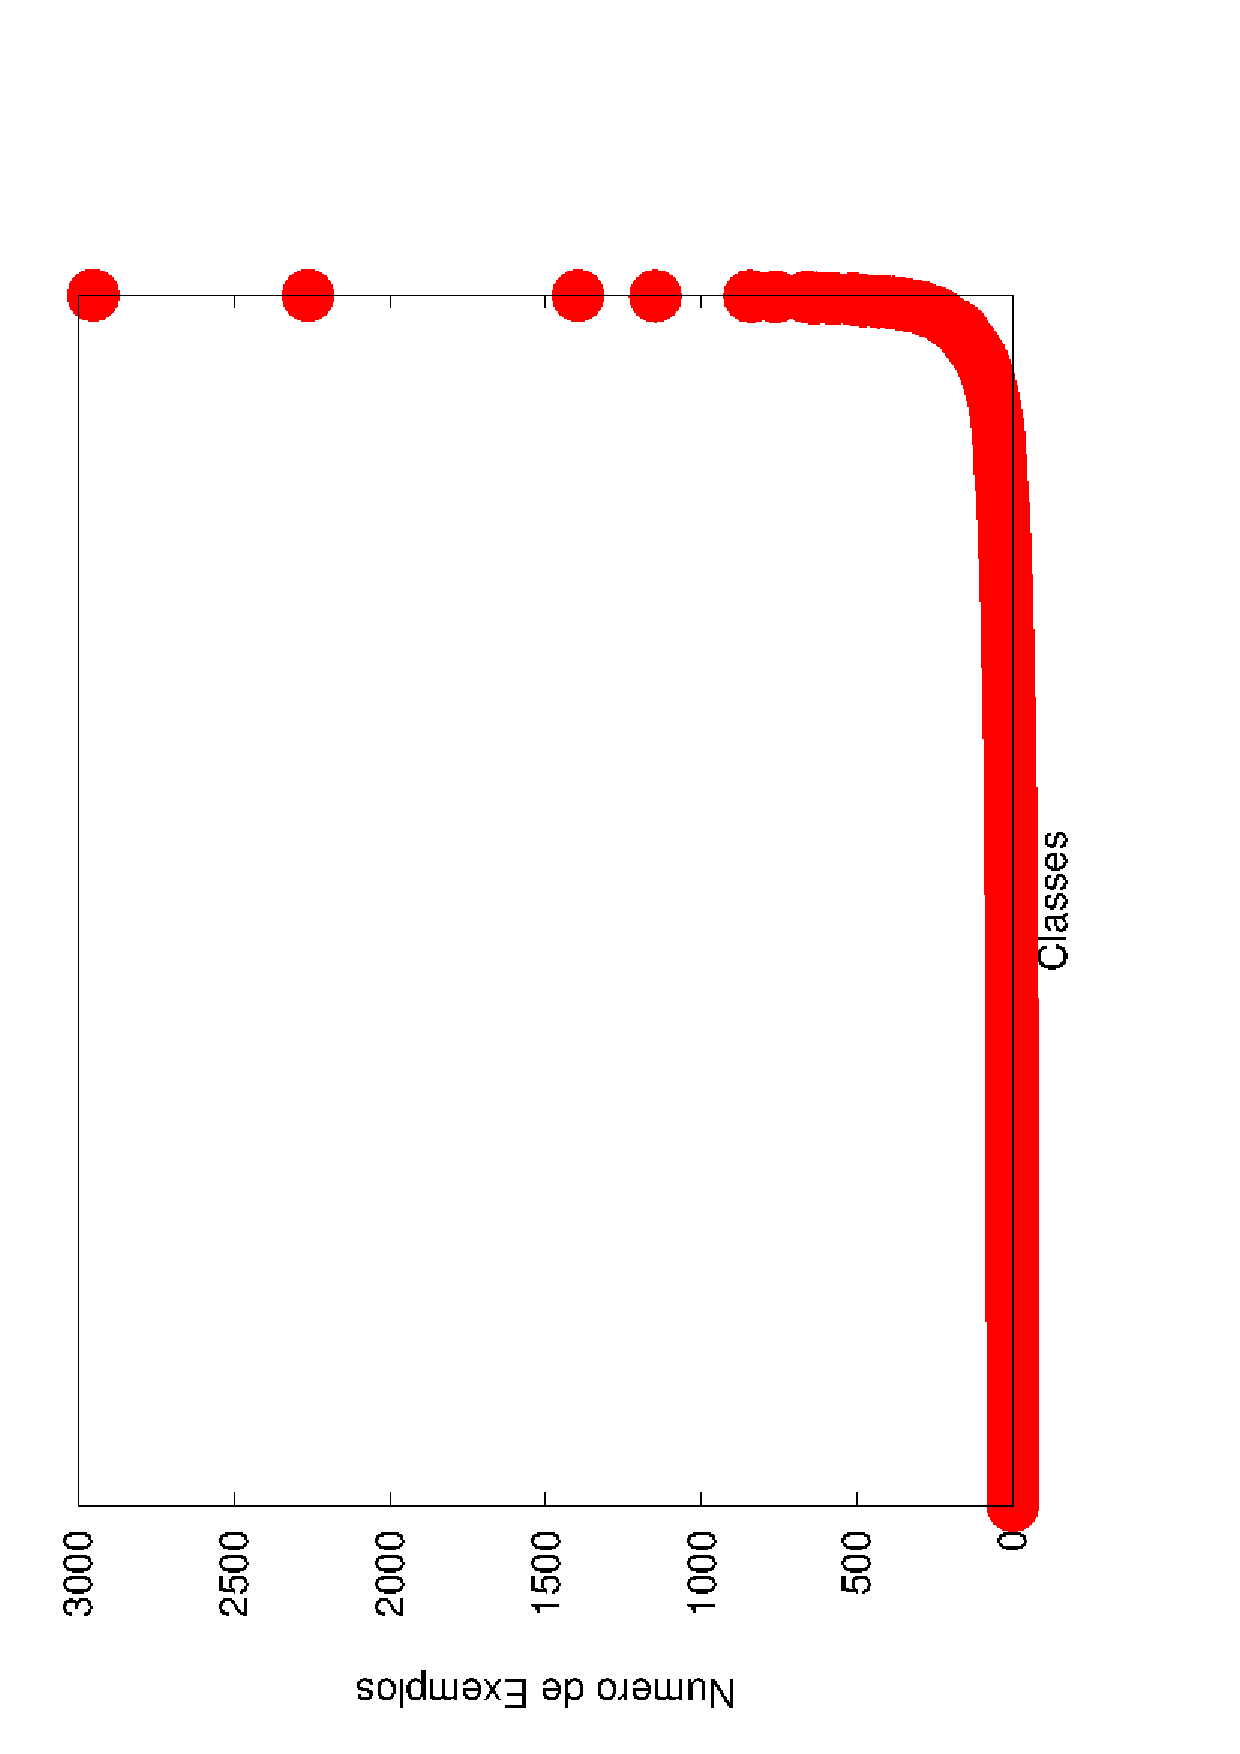
\includegraphics[angle=270, width=0.40\textwidth]{figures/perfil/astral.png}
 \caption{Distribuição de classes na base Astral de bioinformática.}
\label{fig::basesbio}
\end{figure}

%%%%%%%%%%%%%%%%%%%%%%%%%%%%%%%---------------------------------------------------%%%%%%%%%%%%%%%%%%%%%%%%%%%%%%
%%%%%%%%%%%%%%%%%%%%%%%%%%%%%%%---------------------------------------------------%%%%%%%%%%%%%%%%%%%%%%%%%%%%%%
%%%%%%%%%%%%%%%%%%%%%%%%%%%%%%%---------------------------------------------------%%%%%%%%%%%%%%%%%%%%%%%%%%%%%%
%%%%%%%%%%%%%%%%%%%%%%%%%%%%%%%---------------------------------------------------%%%%%%%%%%%%%%%%%%%%%%%%%%%%%%

\subsection{Parâmetros do Programa Genético}


\begin{table}[h]
\centering
\caption{Principais parâmetros utilizados no \textsc{PG}.}
\label{tab::parametros}
%\begin{footnotesize}
\begin{tabular}{|c|c|}
\toprule 
\textbf{Parâmetro} & \textbf{Valor}\tabularnewline
\midrule
Tamanho da Populacão & 100\tabularnewline
\hline 
Número de Geracões & 100\tabularnewline
\hline 
Probabilidade de Cruzamento & 90\tabularnewline
\hline 
Probabilidade de Reproducão & 5\tabularnewline
\hline 
Probabilidade de Cria\'{c}ão & 5\tabularnewline
\hline 
Probabilidade de Mutacão & 10\tabularnewline
\hline 
Tamanho Máximo da Árvore & 6\tabularnewline
\hline 
Tipo de Selecão & Torneio\tabularnewline
\hline 
Elitismo & Sim\tabularnewline
\bottomrule
\end{tabular}
%\end{footnotesize}
\end{table}[h]



\subsection{Efeito da função de \textit{fitness}}
\label{sec::fitness}


Como foi apontado na Seção~\ref{subsec::fitness}, a \textit{fitness} desempenha importante papel em um Programa Genético, pois define quem são os melhores indivíduos, sendo um importante meio de compará-los.
Usualmente, os trabalhos presentes na literatura reportam a Micro e Macro-$F_1$, pelo papel que apresentam em tentar balancear a taxa de acerto com uma boa cobertura, medindo a capacidade do classificador prever corretamente indivíduos em todas as classes.
Em nosso trabalhos passados, sempre utilizamos a Micro-$F_1$ como função de \textit{fitness} (), pelo fato de ser mais comum ver trabalhos reportando a Micro-$F_1$ do que a Macro-$F_1$. Aqui, resolvemos investigar quais são as alterações provocadas pela mudança da função de \textit{fitness} e propomos substituir a Micro-$F_1$ pela Macro-$F_1$ e pela soma das duas, tendendo a dar importância para ambas simultâneamente no processo de evolução.
Nas Tabelas~\ref{tab::fitness-micro} \ref{tab::fitness-macro}... 

\begin{table}[h]
\centering
\caption{Experimentos mostrando a micro$F_1$ variando a função de fitness.}
\label{tab::fitness-micro}
\begin{footnotesize}
\begin{tabular}{|c|c|c|c|c|}
\toprule
\multirow{2}{*}{\textbf{Bases}} & \multirow{2}{*}{\textbf{\textit{Baselines}}} & \multicolumn{3}{c|}{\textbf{Funcão de Fitness}}\tabularnewline
\cline{3-5} 
 &  & \textbf{Micro$F_1$} & \textbf{Macro$F_1$} & \textbf{Macro$F_1$ + Micro$F_1$}\tabularnewline
\midrule
ACM & 73.63 \textpm{} 0.91 & 74.33 \textpm{} 0.72 (0.95 \ball) & 72.96 \textpm{} 0.98 (-0.91 \ball) & 73.99 \textpm{} 0.80 (0.49 \ball)\tabularnewline
\hline 
20NG & 84.94 \textpm{} 0.58 & 89.06 \textpm{} 0.15 (4.85 \triangOK) & 87.92 \textpm{} 1.59 (3.61 \triangOK) & 88.71 \textpm{} 0.14 (4.43 \triangOK)\tabularnewline
\hline 
Ohsumed & 66.56 \textpm{} 0.66 & 69.34 \textpm{} 0.55 (4.19 \triangOK) & 68.83 \textpm{} 1.47 (3.42 \triangOK) & 69.76 \textpm{} 1.19 (4.81 \triangOK)\tabularnewline
\hline 
Reuters & 93.13 \textpm{} 0.29 & 94.60 \textpm{} 0.44 (1.57 \triangOK) & 93.96 \textpm{} 0.78 (0.89 \triangOK) & 94.59 \textpm{} 0.50 (1.56 \triangOK)\tabularnewline
\bottomrule
\end{tabular}
\end{footnotesize}
\end{table}



\begin{table}[h]
\centering
\caption{Experimentos mostrando a macro$F_1$ variando a função de fitness.}
\label{tab::fitness-macro}
\begin{footnotesize}
\begin{tabular}{|c|c|c|c|c|}
\toprule
\multirow{2}{*}{\textbf{Bases}} & \multirow{2}{*}{\textbf{\textit{Baseline}}} & \multicolumn{3}{c|}{\textbf{Funcão de Fitness}}\tabularnewline
\cline{3-5} 
 &  & \textbf{Micro$F_1$} & \textbf{Macro$F_1$} & \textbf{Macro$F_1$ + Micro$F_1$}\tabularnewline
\midrule
ACM & 57.26 \textpm{} 0.93 & 59.72 \textpm{} 1.26 (4.30 \triangOK) & 60.03 \textpm{} 1.45 (4.84 \triangOK) & 60.21 \textpm{} 1.54 (5.15 \triangOK)\tabularnewline
\hline 
20NG & 83.68 \textpm{} 0.82 & 88.69 \textpm{} 0.22 (5.99 \triangOK) & 86.46 \textpm{} 3.80 (3.39 \triangOK) & 88.34 \textpm{} 0.06 (5.57 \triangOK)\tabularnewline
\hline 
Ohsumed & 54.76 \textpm{} 1.27 & 63.56 \textpm{} 0.90 (16.06 \triangOK) &  63.62 \textpm{} 1.88 (16.18 \triangOK) & 64.38 \textpm{} 1.90 (17.57 \triangOK)\tabularnewline
\hline 
Reuters & 81.96 \textpm{} 1.44 & 89.33 \textpm{} 0.90 (8.99 \triangOK) & 88.04 \textpm{} 0.73 (7.42 \triangOK) & 89.08 \textpm{} 0.83 (8.69 \triangOK)\tabularnewline
\bottomrule
\end{tabular}
\end{footnotesize}
\end{table}




%%%%%%%%%%%%%%%%%%-------%%%%%%%%%%%%%%%
%%%%%%%%%%%%%%%%%%-------%%%%%%%%%%%%%%%

\section{Bases de Documentos}
\label{sec::documentos}

\begin{table}[h]
\renewcommand{\arraystretch}{1.3}
\centering
\caption{Funções de credibilidade geradas para cada uma das bases.}
\label{tab::}
\begin{scriptsize}
\begin{tabular}{|c|c|}
\toprule
\textbf{Base} & \textbf{Função de Credibilidade}\tabularnewline
\midrule
ACM   & $F_{ACM} =  DOM^{(GSS)^{(CE + TF)}} $\tabularnewline
\hline 
20NG & $F_{20NG} = DF + MaxAM + (\dfrac{ CHI } { TFIDF^{(MaxTFIDF)} }) $\tabularnewline
\hline 
Ohsumed  & $ F_{Ohsumed} = (\dfrac{AM}{MaxIG \times CC^{(sumDF)}} )^{(TFICF)^{(TFICF)}} $\tabularnewline
\hline 
Reuters & $ F_{Reuters} = IG^{(MaxIG \times GINI)}$\tabularnewline
\bottomrule
\end{tabular}
\end{scriptsize}
\end{table}

\begin{table}[h]
\centering
\caption{Micro$F_1$ obtida pelo \textit{Naïve Bayes} quando usando a função de credibilidade $F_base$ gerada uma dada base nas demais bases.}
\label{tab::generalizacao-Micro}
\begin{scriptsize}
\begin{tabular}{|c||c|c|c|c|}
\toprule
\textbf{Funções evoluídas} & \textbf{ACM} & \textbf{Reuters} & \textbf{Ohsumed} & \textbf{20NG}\tabularnewline
\midrule
\textit{Baselines} & 73.63 \textpm{} 0.91 & 93.13 \textpm{} 0.29 & 66.56 \textpm{} 0.66 & 84.86 \textpm{} 0.54\tabularnewline
\hline 
$F_{ACM}$ & 75.04 \textpm{} 0.88 (1.91 \triangOK) & 92.68 \textpm{} 0.45 (-0.48 \triangBAD) & 66.06 \textpm{} 0.59 (-0.75 \ball) & 84.45 \textpm{} 0.35 (-0.49 \triangBAD)\tabularnewline
\hline 
$F_{20ng}$ & 66.69 \textpm{} 0.65 (-9.42 \triangBAD) & 94.01 \textpm{} 0.53 (0.94 \triangOK) & 67.94 \textpm{} 0.62 (2.08 \triangOK)  & 88.97 \textpm{} 0.17 (4.84 \triangOK)\tabularnewline
\hline 
$F_{Ohsumed}$ & 70.09 \textpm{} 0.82 (-4.81 \triangBAD) & 93.45 \textpm{} 0.57 (0.34 \ball) & 69.54 \textpm{} 0.69 (4.49 \triangOK) & 85.60 \textpm{} 0.27 (0.87 \triangOK)\tabularnewline
\hline 
$F_{Reuters}$ & 66.55 \textpm{} 0.89 (-9.61 \triangBAD) & 94.87 \textpm{} 0.25 (1.86 \triangOK) & 63.32 \textpm{} 0.82 (-4.86 \triangBAD) & 87.04 \textpm{} 0.41 (2.57 \triangOK)\tabularnewline
\bottomrule
\end{tabular}
\end{scriptsize}
\end{table}


\begin{table}[h]
\centering
\caption{Macro$F_1$ obtida pelo \textit{Naïve Bayes} quando usando a função de credibilidade $F_base$ gerada uma dada base nas demais bases.}
\label{tab::generalizacao-Macro}
\begin{scriptsize}
\begin{tabular}{|c||c|c|c|c|}
\toprule
\textbf{Funções evoluídas} & \textbf{ACM} & \textbf{Reuters} & \textbf{Ohsumed} & \textbf{20NG}\tabularnewline
\midrule
\textit{Baselines} & 57.26 \textpm{} 0.93 & 81.96 \textpm{} 1.44 & 54.76 \textpm{} 1.27 & 83.62 \textpm{} 0.74\tabularnewline
\hline 
$F_{ACM}$ & 60.13 \textpm{} 1.44 (5.02 \triangOK) & 85.49 \textpm{} 0.94 (4.31 \triangOK) & 56.41 \textpm{}  0.92 (3.00 \triangOK) & 82.88 \textpm{} 0.51 (-0.89 \triangBAD)\tabularnewline
\hline 
$F_{20NG}$ & 55.83 \textpm{} 0.66 (-2.50 \triangBAD) & 88.64 \textpm{} 1.03 (8.16 \triangOK) & 62.12 \textpm{} 1.41 (13.43 \triangOK) & 88.63 \textpm{} 0.18 (5.99 \triangOK)\tabularnewline
\hline 
$F_{Ohsumed}$ & 57.59 \textpm{} 0.56 (0.58 \ball) & 87.41 \textpm{} 0.64 (6.65 \triangOK) & 64.35 \textpm{} 1.17 (17.51 \triangOK) & 84.26 \textpm{}  0.49 (0.77 \triangOK)\tabularnewline
\hline 
$F_{Reuters}$ & 54.84 \textpm{} 1.44 (-4.23\triangBAD) & 89.45 \textpm{}  0.74 (9.14 \triangOK) & 57.97 \textpm{} 1.59 (5.85 \triangOK) & 83.15 \textpm{} 2.04 (-0.56 \ball)\tabularnewline
\bottomrule
\end{tabular}
\end{scriptsize}
\end{table}

%%%%%%%%%%%%%%%%%%-------%%%%%%%%%%%%%%%
%%%%%%%%%%%%%%%%%%-------%%%%%%%%%%%%%%%

\subsection{Explorando múltiplos fatores.}
\label{subsec::fatores}

\begin{table}[h]
\centering
\caption{Resultados do uso de credibilidade na base da \textsc{ACM} explorando a credibilidade de termos, autoria e citação.}
\label{tab::fatores}
\begin{footnotesize}
\begin{tabular}{|c|c|c|c|c|}
\toprule
\textbf{Termos} & \textbf{Autoria} & \textbf{Citação} & \textbf{Micro$F_1$} & \textbf{Macro$F_1$}\tabularnewline
\midrule
\multicolumn{3}{|c|}{Baseline} & 73.63 \textpm{} 0.91 & 57.26 \textpm{} 0.93\tabularnewline
\hline 
X &  &  & 74.33 \textpm{} 0.72 (0.95 \ball) & 59.72 \textpm{} 1.26 (4.30 \triangOK)\tabularnewline
\hline 
 & X &  & 76.19 \textpm{} 0.82 (3.48 \triangOK) & 60.37 \textpm{} 0.70 (5.43 \triangOK)\tabularnewline
\hline 
 &  & X & 75.58 \textpm{} 0.85 (2.65 \triangOK) & 59.00 \textpm{} 0.90 (3.04 \triangOK)\tabularnewline
\hline 
X & X &  & 76.70 \textpm{} 1.08 (4.18 \triangOK) & 61.82 \textpm{} 1.38 (7.96 \triangOK)\tabularnewline
\hline 
X &  & X & 75.63 \textpm{} 1.03 (2.72 \triangOK) & 60.69 \textpm{} 1.30 (5.98 \triangOK)\tabularnewline
\hline 
 & X & X & 77.29 \textpm{} 0.79 (4.98 \triangOK) & 61.41 \textpm{} 0.65 (7.25 \triangOK)\tabularnewline
\hline 
X & X & X & 77.01 \textpm{} 0.98 (4.60 \triangOK) & 62.24 \textpm{} 1.01 (8.70 \triangOK)\tabularnewline
\bottomrule
\end{tabular}
\end{footnotesize}
\end{table}

%%%%%%%%%%%%%%%%%%-------%%%%%%%%%%%%%%%
%%%%%%%%%%%%%%%%%%-------%%%%%%%%%%%%%%%
%%%%%%%%%%%%%%%%%%-------%%%%%%%%%%%%%%%

\section{Bases de Categorias.}
\label{sec::categorias}


\begin{table}[h]
\centering
\caption{Resultados da Micro$F_1$ para as bases de atributos categóricos}
\label{tab::cat-micro}
\begin{footnotesize}
\begin{tabular}{|c|c|c|c|c|}
\toprule
\multirow{2}{*}{\textbf{Bases}} & \multicolumn{2}{c|}{\textbf{Naïve Bayes}} & \multicolumn{2}{c|}{\textbf{KNN}}\tabularnewline
\cline{2-5} 
 & \textbf{\textit{Baselines}} & \textbf{Macro$F_1$} & \textbf{\textit{Baselines}} & \textbf{Macro$F_1$}\tabularnewline
\midrule
Cars & 67.74 \textpm{} 3.08 & 76.85 \textpm{} 5.65 (13.44 \triangOK) & 75.36 \textpm{} 3.44 & 81.77 \textpm{} 3.90 (8.51 \triangOK)\tabularnewline
\hline 
TicTacToe & 64.48 \textpm{} 2.12 & 64.10 \textpm{} 1.96 (-0.59 \ball) & 95.99 \textpm{} 0.98 & 97.12 \textpm{} 1.10 (1.18 \ball)\tabularnewline
\hline 
Nusery & 66.19 \textpm{} 7.41 & 77.19 \textpm{} 12.80 (16.62 \triangOK) & 95.84 \textpm{} 0.73 & 96.00 \textpm{} 0.69 (0.17 \ball) \tabularnewline
\hline 
Chess & 87.81 \textpm{} 0.68 & 88.03 \textpm{} 0.75 (0.25 \ball) & 94.75 \textpm{} 0.40  & 95.98 \textpm{} 0.61 (1.30 \triangOK)\tabularnewline
\bottomrule
\end{tabular}
\end{footnotesize}
\end{table}


 	
\begin{table}[h]
\centering
\caption{Resultados da Macro$F_1$ para as bases de atributos categóricos}
\label{tab::cat-macro}
\begin{footnotesize}
\begin{tabular}{|c|c|c|c|c|}
\toprule
\multirow{2}{*}{\textbf{Bases}} & \multicolumn{2}{c|}{\textbf{Naïve Bayes}} & \multicolumn{2}{c|}{\textbf{KNN}}\tabularnewline
\cline{2-5} 
 & \textbf{\textit{Baselines}} & \textbf{Micro$F_1$} & \textbf{\textit{Baselines}} & \textbf{Micro$F_1$}\tabularnewline
\midrule
Cars & 86.32 \textpm{} 1.85 & 87.64 \textpm{} 2.53 (1.52 \triangOK) & 91.84 \textpm{} 1.95 & 92.43 \textpm{} 1.68 (0.64 \ball)\tabularnewline
\hline 
TicTacToe & 70.63 \textpm{} 2.10 & 71.74 \textpm{} 2.02 (1.58 \triangOK) & 96.45 \textpm{} 0.85  & 97.42 \textpm{} 0.94 (1.00 \ball)\tabularnewline
\hline 
Nusery & 90.29 \textpm{} 0.56 & 91.21 \textpm{} 0.92 (1.01 \ball) & 80.83 \textpm{} 9.06  &	84.46 \textpm{} 9.22 (4.50 \triangOK) \tabularnewline
\hline 
Chess & 87.85 \textpm{} 0.69 & 88.04 \textpm{} 0.75 (0.21 \ball) & 94.77 \textpm{} 0.41  & 96.00 \textpm{} 0.60 (1.29 \triangOK)\tabularnewline
\bottomrule
\end{tabular}
\end{footnotesize}
\end{table}


%%%%%%%%%%%%%%%%%%-------%%%%%%%%%%%%%%%
%%%%%%%%%%%%%%%%%%-------%%%%%%%%%%%%%%%
%%%%%%%%%%%%%%%%%%-------%%%%%%%%%%%%%%%


\section{Bases de BioInformática.}
\label{sec::bioinfo}

\begin{table}
\centering
\caption{asdfsa}
\label{tab::}
\begin{scriptsize}
\begin{tabular}{|c|c|c|c|c|c|c|c|c|c|}
\toprule & ACM - micro & ACM - macro &  & Reuters - micro & Reuters - macro &  &  &  & \tabularnewline
\midrule
Baseline & 73.6274, 2.023 & 57.2580, 2.083 &  & 93.13 \textpm{} 0.29 & 81.96 \textpm{} 1.44 &  &  &  & \tabularnewline
\hline 
GP & 74.33 \textpm{} 0.72 (0.95 \ball) & 59.72 \textpm{} 1.26 (4.30 \triangOK) &  & 94.60 \textpm{} 0.44 (1.57 \triangOK) & 89.33 \textpm{} 0.90 (8.99 \triangOK) &  &  &  & \tabularnewline
\hline 
AM & 73.13, 1.05 (-0.68 \triangBAD) & 58.02, 1.73 (1.33 \ball) &  & 93.43, 0.38 (0.31 \ball) & 85.28, 0.87 (4.06 \triangOK) &  &  &  & \tabularnewline
\hline 
CC & 69.69, 0.70 (-5.35 \triangBAD) & 56.93, 0.90 (-0.57 \ball) &  & 93.58, 0.55 (0.66 \ball) & 88.56, 0.02 (7.31 \triangOK)  &  &  &  & \tabularnewline
\hline 
CE & 44.65, 0.34 (-39.35 \triangBAD) & 22.94, 0.41 (-59.93 \triangBAD) &  & 76.72, 0.44 (-17.67 \triangBAD) & 31.55, 1.48 (-61.73 \triangBAD) &  &  &  & \tabularnewline
\hline 
CHI & 69.86, 0.74 (-5.12 \triangBAD) & 56.81, 1.00 (-0.78 \ball) &  & 93.76, 0.54 (0.67 \triangOK) & 88.31, 0.95 (7.75 \triangOK) &  &  &  & \tabularnewline
\hline 
CTD & 58.75, 1.83 (-20.20 \triangBAD) & 50.63, 0.97 (-11.58 \triangBAD) &  & 72.41, 1.73 (-22.25 \triangBAD) & 66.44, 1.50 (-18.93 \triangBAD) &  &  &  & \tabularnewline
\hline 
DF & 66.81, 0.64 (-9.26 \triangBAD) & 55.83, 0.57 (-2.50 \triangBAD) &  & 92.79, 0.77 (-0.37 \ball) & 87.24, 0.98 (6.44 \triangOK) &  &  &  & \tabularnewline
\hline 
DOM & 73.38, 0.97 (-0.33 \triangBAD) & 58.34, 1.62 (1.89 \ball) &  & 93.43, 0.38 (0.31 \ball) & 85.28, 0.87 (4.06 \triangOK) &  &  &  & \tabularnewline
\hline 
GINI & 71.35, 0.77 (-3.10 \triangBAD) & 58.11, 1.00 (1.49 \triangOK) &  & 92.45, 0.60 (-0.73 \ball)  & 86.58, 0.95 (5.63 \triangOK) &  &  &  & \tabularnewline
\hline 
GSS & 69.65, 0.71 (-5.40 \triangBAD) & 56.90, 0.91 (-0.62 \ball) &  & 93.77, 0.54 (0.68 \triangOK) & 88.43, 0.91 (7.90 \triangOK) &  &  &  & \tabularnewline
\hline 
IDF & 58.75, 1.83 (-20.20 \triangBAD) & 50.63, 0.97 (-11.58 \triangBAD) &  & 72.41, 1.73 (-22.25 \triangBAD) & 66.44, 1.50 (-18.93 \triangBAD) &  &  &  & \tabularnewline
\hline 
IG & 71.31, 0.65 (-3.15 \triangBAD) & 58.06, 1.04 (1.41 \triangOK) &  & 94.04, 0.46 (0.97 \triangOK) & 88.88, 0.93 (8.44 \triangOK) &  &  &  & \tabularnewline
\hline 
MaxAM & 72.17, 0.67 (-1.97 \triangBAD) & 58.64, 1.20 (2.41 \triangOK) &  & 92.73, 0.64 (-0.43 \ball) & 87.07, 0.95 (6.23 \triangOK) &  &  &  & \tabularnewline
\hline 
MaxCC & 1.49, 0.05 (-97.98 \triangBAD) & 0.27, 0.01 (-99.52 \triangBAD) &  & 5.22, 0.05 (-94.40 \triangBAD) & 1.32, 0.18 (-98.39 \triangBAD) &  &  &  & \tabularnewline
\hline 
MaxCHI & 68.41, 0.58 (-7.09 \triangBAD) & 56.22, 0.64 (-1.8 \triangBAD) &  & 93.22, 0.81 (0.09 \ball) & 87.43, 1.22 (6.68 \triangOK) &  &  &  & \tabularnewline
\hline 
MaxCTD & 37.69, 2.08 (-48.81 \triangBAD) & 38.29, 1.43 (-33.13 \triangBAD) &  & 61.78, 1.59 (-33.67 \triangBAD) & 54.09, 0.96 (-34.01 \triangBAD) &  &  &  & \tabularnewline
\hline 
MaxDom & 72.25, 0.70 (-1.87 \triangBAD) & 58.74, 1.27 (2.58 \triangOK) &  & 92.73, 0.64 (-0.43 \ball) & 87.07, 0.95 (6.23 \triangOK) &  &  &  & \tabularnewline
\hline 
MaxGSS & 1.48, 0.06 (-97.99 \triangBAD) & 0.26, 0.01 (-99.54 \triangBAD) &  & 5.19, 0.04 (-94.42 \triangBAD) & 1.23, 0.01 (-98.49 \triangBAD) &  &  &  & \tabularnewline
\hline 
MaxIG & 68.49, 0.60 (-6.98 \triangBAD) & 56.42, 0.63 (-1.47 \ball) &  & 93.61, 0.70 (0.51 \ball) & 88.05, 1.01 (7.43 \triangOK) &  &  &  & \tabularnewline
\hline 
MaxOR & 48.15, 0.43 (-34.60 \triangBAD) & 28.15, 0.74 (-50.83 \triangBAD) &  & 79.99, 0.27 (-14.12 \triangBAD) & 40.94, 1.06 (-50.04 \triangBAD) &  &  &  & \tabularnewline
\hline 
OR & 68.54, 0.95 (-6.91 \triangBAD) & 56.80, 1.22 (-0.80 \ball) &  & 92.42, 0.59 (-0.76 \triangBAD) & 86.67, 0.56 (5.75 \triangOK) &  &  &  & \tabularnewline
\hline 
P & 72.96, 1.06 (-0.90 \triangBAD) & 57.51, 1.54 (0.44 \ball) &  & 93.32, 0.38 (0.20 \ball) & 84.92, 0.81 (3.61 \triangOK) &  &  &  & \tabularnewline
\hline 
TF & 66.16, 5.91 (-10.14 \triangBAD) & 54.89, 3.33 (-4.14 \ball) &  & 86.32, 9.91 (-7.31 \ball) & 79.64, 9.43 (-2.83 \ball) &  &  &  & \tabularnewline
\hline 
TFICF & 58.75, 1.83 (-20.20 \triangBAD) & 50.63, 0.97 (-11.58 \triangBAD) &  & 72.41, 1.73 (-22.25 \triangBAD) & 66.44, 1.50 (-18.93 \triangBAD) &  &  &  & \tabularnewline
\hline 
TFIDF & 72.84, 1.05 (-1.06 \triangBAD) & 58.33, 1.08 (1.87 \triangOK) &  & 93.77, 0.36, (0.68 \triangOK) & 85.25, 0.64 (4.01 \triangOK) &  &  &  & \tabularnewline
\hline 
sumTF & 66.93, 0.85 (-9.09 \triangBAD) & 55.57, 0.72 (-2.95 \triangBAD) &  & 92.80, 0.75 (-0.35 \ball) & 87.56, 1.55 (6.84 \triangOK) &  &  &  & \tabularnewline
\hline 
sumDF & 66.99, 0.82 (-9.02 \triangBAD) & 55.60, 0.70 (-2.89 \triangBAD)  &  & 92.80, 0.75 (-0.35 \ball) & 87.56, 1.55 (6.84 \triangOK)  &  &  &  & \tabularnewline
\hline 
 &  &  &  &  &  &  &  &  & \tabularnewline
\hline 
 &  &  &  &  &  &  &  &  & \tabularnewline
\hline 
 &  &  &  &  &  &  &  &  & \tabularnewline
\hline 
 &  &  &  &  &  &  &  &  & \tabularnewline
\bottomrule

\end{tabular}
\end{scriptsize}
\end{table}


 	

